\documentclass{prettytex/ox/mmsc-special-topic}
\usepackage{tabularray}
\usepackage{pdfpages}
\setlength{\headheight}{19.53pt}

\setcounter{biburllcpenalty}{7000}
\setcounter{biburlucpenalty}{8000}

\addbibresource{sources.bib}
\tikzexternalize[prefix=tikz/]

\newcommand{\topictitle}{
  Melon - a Task Scheduling Package for Personal Todo Lists \\
  \normalsize using Markov Chain Monte-Carlo Methods
}
\newcommand{\candidatenumber}{1072462}
\newcommand{\course}{Python in Scientific Computing}

\title{\topictitle}
\author{Candidate \candidatenumber}
\date{\today}

\makenoidxglossaries
\newacronym{ode}{ODE}{Ordinary Differential Equation}
\newacronym{pde}{PDE}{Partial Differential Equation}
\newacronym{gui}{GUI}{Graphical User Interface}

\begin{document}
  \pagestyle{plain}
  \mmscSpecialHeader

  \begin{abstract}
    \label{abstract}
    In this project report we will review the central concepts utilised in the group work conducted to make progress in the \gls{pde} problem associated with the electrochemical model of a battery cell and present numerical results.
    \vspace*{0.2cm}

    \noindent
    \textbf{Our Goal:}
    Numerically obtain the solution $\{a(x, T), b(x, T)\}$.

    The Finite Difference schemes are implemented in Julia and Python, whereas the Spectral Method is implemented in C++.
  \end{abstract}

  \begin{figure}[H]
    \centering
    % \includegraphics[width=\linewidth]{figures/screenshot.png}
    \caption{The \gls{gui} of the Spectral Solver.}
    \label{fig:gui}
  \end{figure}

  \pagebreak
  \pagestyle{normal}

  \section{Problem Introduction}
  \label{sec:introduction}

  UIDs are useful because they make collisions very unlikely, which is not to say that these should not be checked, but if two clients are connected that each generated a set of UIDs it is very unlikely to have to do conflict resolving.

  We recommend usage with \texttt{xandikos}, a version-controlled DAV server, capable of syncing calendars (events, todos and journals) and contacts.

  Published on PyPi.

  \subsection{Usage}
  % TODO: describe installation, etc., running main.py
  Use \texttt{invoke -l} to list all available tasks.

  Is platform-independent, for example due to the usage of \texttt{pathlib.Path}.

  \section{Code Quality}
  \subsection{Formatting}
  \subsection{Docstrings}
  \subsection{Documentation}
  \subsection{Tests}
  Server can be started using Docker.

  \subsubsection{Coverage}
  \subsection{Type Checking}
  Using \texttt{pyright} instead of \texttt{mypy} as it is much faster.
  \subsection{Using Appropriate Language Features}
  Using \texttt{autoflake} and \texttt{pyupgrade}.
  Used \texttt{logging}.
  \subsection{Maintaining Code Quality}
  Using \texttt{pre-commit} and GitHub Actions CI/CD.
  Uses \texttt{invoke} to manage common development tasks.

  \begin{minted}{python}
    import numpy
    x = 5
    print(x ** 2)
  \end{minted}

  interrogate -v einfügen

  Screenshot von gnome-calendar

  Screenshot GUI

  \subsection{Autocorrelation Analysis}
  \subsection{Coole Pie-Plots mit Verteilungen}

  \section{Runtime Performance}
  \begin{minted}{python}
In [1]: %timeit str(t.icalendar_component["uid"])
  122 µs ± 1.06 µs per loop (7 runs, 10,000 loops each)
In [2]: %timeit t.vtodo.contents["uid"][0].value
  355 ns ± 7.14 ns per loop (7 runs, 1,000,000 loops each)
In [3]: %timeit t.vobject_instance.contents["vtodo"][0].contents["uid"][0].value
  296 ns ± 7.06 ns per loop (7 runs, 1,000,000 loops each)
In [4]: %timeit t._vobject_instance.contents["vtodo"][0].contents["uid"][0].value
  208 ns ± 23.7 ns per loop (7 runs, 10,000,000 loops each)
  \end{minted}

  \begin{table}[H]
    \centering
    \caption{Profile obtained by running \mintinline{bash}{./main.py --profile | grep todo.py}.}
    \begin{tabular}{rrrrrll}
      16958 & 0.008 & 0.000 & 0.939 & 0.000 & todo.py:36  & vtodo        \\
      32475 & 0.047 & 0.000 & 0.705 & 0.000 & todo.py:96  & uid          \\
      856   & 0.003 & 0.000 & 0.579 & 0.001 & todo.py:26  & upgrade      \\
      117   & 0.000 & 0.000 & 0.489 & 0.004 & todo.py:111 & priority     \\
      417   & 0.001 & 0.000 & 0.461 & 0.001 & todo.py:121 & isIncomplete \\
      5512  & 0.003 & 0.000 & 0.278 & 0.000 & todo.py:45  & summary      \\
      856   & 0.002 & 0.000 & 0.112 & 0.000 & todo.py:21  & \_\_init\_\_ \\
      1363  & 0.006 & 0.000 & 0.024 & 0.000 & todo.py:164 & \_\_lt\_\_   \\
      7844  & 0.004 & 0.000 & 0.009 & 0.000 & todo.py:61  & dueDate      \\
      2605  & 0.001 & 0.000 & 0.003 & 0.000 & todo.py:85  & dueTime      \\
    \end{tabular}
  \end{table}

  \section{Results}
  \begin{figure}[H]
    \centering
    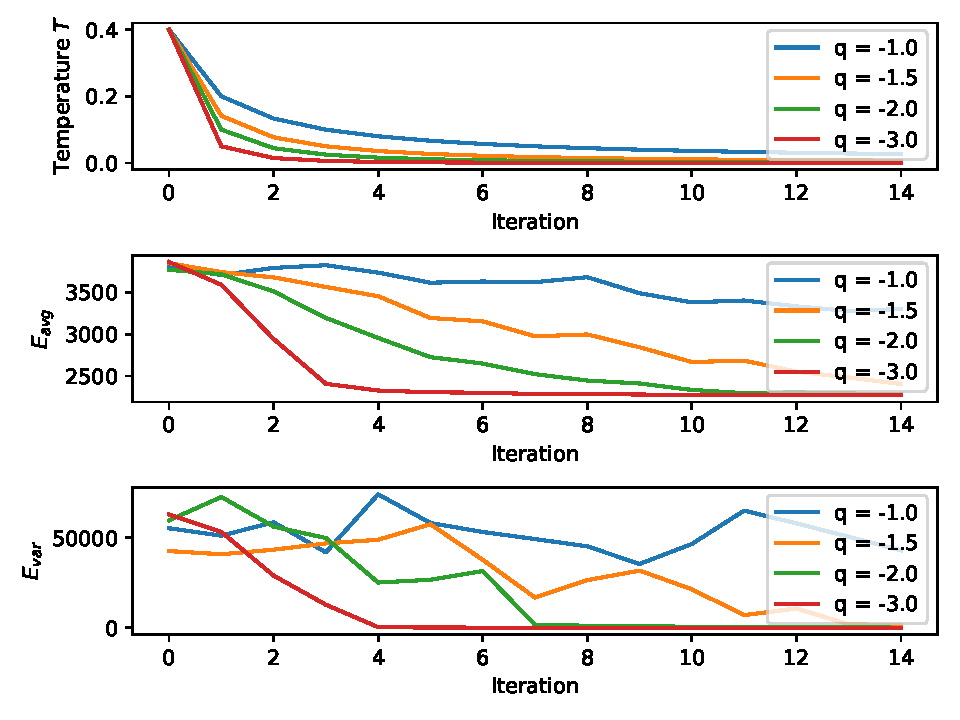
\includegraphics[width=0.8\linewidth]{results/convergence.pdf}
    \caption{Convergence}
  \end{figure}

  \section{Acknowledgements}
  The visualisation code (\texttt{visualise.py}) is adapted from \cite{monte-carlo-todo-lists}.

  The task check icon is the logo of the \textit{Tasks.org} Free and Open Source Android App, which may be found \href{https://github.com/tasks/tasks/tree/main/graphics}{here}.

  \pagebreak
  \printbibliography
  \printnoidxglossary[type=acronym]

  % \appendix
\end{document}
